% =============================================================================
% Nerve 1.0 -- Technical Reference Manual
% Copyright (C) 2025 Fatih Kucukkarakurt
% SPDX-License-Identifier: GPL-3.0-or-later
%
% Compile:
%   pdflatex nerve_manual.tex
%   bibtex   nerve_manual
%   pdflatex nerve_manual.tex
%   pdflatex nerve_manual.tex
% =============================================================================

\documentclass[11pt,a4paper]{article}

% --------------------------------------------------------------------------- %
%  Encoding & fonts
% --------------------------------------------------------------------------- %
\usepackage[utf8]{inputenc}
\usepackage[T1]{fontenc}
\usepackage{lmodern}
\usepackage{microtype}

% --------------------------------------------------------------------------- %
%  Mathematics
% --------------------------------------------------------------------------- %
\usepackage{amsmath,amssymb,amsthm}
\usepackage{mathtools}
\usepackage{bm}

% --------------------------------------------------------------------------- %
%  Algorithms
% --------------------------------------------------------------------------- %
\usepackage[ruled,vlined,linesnumbered]{algorithm2e}

% --------------------------------------------------------------------------- %
%  Tables
% --------------------------------------------------------------------------- %
\usepackage{booktabs}
\usepackage{array}
\usepackage{multirow}
\usepackage{tabularx}

% --------------------------------------------------------------------------- %
%  Graphics & diagrams
% --------------------------------------------------------------------------- %
\usepackage{tikz}
\usetikzlibrary{positioning,arrows.meta,calc,fit,backgrounds}
\usepackage{pgfplots}
\pgfplotsset{compat=1.18}

% --------------------------------------------------------------------------- %
%  Page layout
% --------------------------------------------------------------------------- %
\usepackage[top=2.8cm,bottom=2.8cm,left=3cm,right=3cm]{geometry}
\usepackage{setspace}
\setstretch{1.12}
\usepackage{parskip}
\setlength{\parskip}{6pt}

% --------------------------------------------------------------------------- %
%  Code listings
% --------------------------------------------------------------------------- %
\usepackage{listings}
\usepackage{xcolor}
\definecolor{codebg}{rgb}{0.97,0.97,0.97}
\definecolor{kwcolor}{rgb}{0.0,0.0,0.65}
\definecolor{cmtcolor}{rgb}{0.40,0.40,0.40}
\definecolor{strcolor}{rgb}{0.10,0.45,0.10}
\lstdefinestyle{nerve}{
  language=C,
  basicstyle=\ttfamily\footnotesize,
  backgroundcolor=\color{codebg},
  keywordstyle=\color{kwcolor}\bfseries,
  commentstyle=\color{cmtcolor}\itshape,
  stringstyle=\color{strcolor},
  numbers=left, numberstyle=\tiny\color{gray},
  numbersep=6pt,
  frame=single, framerule=0.4pt,
  breaklines=true, breakatwhitespace=true,
  captionpos=b, aboveskip=8pt, belowskip=6pt
}
\lstset{style=nerve}

% --------------------------------------------------------------------------- %
%  Bibliography
% --------------------------------------------------------------------------- %
\usepackage[numbers,sort&compress]{natbib}

% --------------------------------------------------------------------------- %
%  Hyperlinks
% --------------------------------------------------------------------------- %
\usepackage[colorlinks=true,
            linkcolor=blue!60!black,
            citecolor=blue!60!black,
            urlcolor=blue!60!black]{hyperref}

% --------------------------------------------------------------------------- %
%  Misc
% --------------------------------------------------------------------------- %
\usepackage{caption}
\usepackage{subcaption}
\usepackage{float}
\usepackage{enumitem}
\usepackage{abstract}

% --------------------------------------------------------------------------- %
%  Theorem environments
% --------------------------------------------------------------------------- %
\newtheorem{proposition}{Proposition}[section]
\newtheorem{remark}{Remark}[section]
\newtheorem{definition}{Definition}[section]

% --------------------------------------------------------------------------- %
%  Custom commands
% --------------------------------------------------------------------------- %
\newcommand{\nerve}{\textsc{Nerve}}
\newcommand{\R}{\mathbb{R}}
\newcommand{\norm}[1]{\left\lVert#1\right\rVert}
\DeclareMathOperator*{\argmax}{arg\,max}

% ============================================================================ %
%  TITLE
% ============================================================================ %
\title{%
  \textbf{\Large \nerve{} 1.0}\\[0.5em]
  \large Technical Reference Manual\\[0.3em]
  \normalsize\itshape
  A Zero-Dependency Single-Header Multilayer Perceptron Library for ANSI C%
}

\author{%
  Fatih K\"{u}\c{c}\"{u}kkarakurt\\[0.4em]
  \small Independent Researcher\\[0.1em]
  \small \href{https://github.com/fkkarakurt}{\texttt{https://github.com/fkkarakurt}}
}

\date{Version 2.0.0\quad\textbullet\quad 2025}

% ============================================================================ %
\begin{document}
% ============================================================================ %

\maketitle
\thispagestyle{empty}
\vspace{1em}

% --------------------------------------------------------------------------- %
\begin{abstract}
\noindent
We present \nerve{}, a multilayer perceptron (MLP) library implemented in ANSI
C as a single, self-contained header file. The library requires no external
dependencies and integrates into any C or C\texttt{++} project by copying one
file. \nerve{} implements the full supervised-learning pipeline: forward
propagation, mean-squared-error loss, and backpropagation as formulated by
\citeauthor{rumelhart1986}~\cite{rumelhart1986}. Two first-order optimizers are
provided---stochastic gradient descent with momentum and the Adam adaptive
moment estimator~\cite{kingma2015}---together with Xavier/Glorot and He weight
initialization~\cite{glorot2010,he2015}, four activation functions (logistic
sigmoid, hyperbolic tangent, ReLU, and Leaky ReLU~\cite{nair2010,maas2013}),
L2 weight decay, and inverted dropout~\cite{srivastava2014}. A high-level
\emph{Easy API} allows network construction from a topology string (e.g.\
\texttt{"2->8->1"}) and single-call training. Experimental evaluation on
canonical benchmarks demonstrates that Adam reduces convergence iterations by
up to $18.7\times$ relative to vanilla SGD on a 4-class identity problem;
the Iris dataset is classified at $96.7\%$ test accuracy; and a three-class
non-linearly separable spiral achieves $98.3\%$ accuracy with a
2\textendash32\textendash32\textendash3 architecture. The library is released
under the GNU General Public License~v3.
\end{abstract}

\vspace{0.5em}
\newpage
\tableofcontents
\newpage

% ============================================================================ %
\section{Introduction}
% ============================================================================ %

The multilayer perceptron~\cite{rumelhart1986,rosenblatt1958} remains the
canonical supervised-learning model: a directed acyclic graph of parametric
neurons, organized into layers, trained by gradient descent through
backpropagation. Despite decades of research and the proliferation of
high-level deep-learning frameworks, a recurring practical need exists for
a \emph{minimal}, \emph{portable}, and \emph{dependency-free} MLP
implementation suitable for embedded systems, game engines, real-time
industrial control, and educational contexts where linking against TensorFlow,
PyTorch, or ONNX Runtime is infeasible.

\nerve{} addresses this need. Its entire implementation---data structures,
forward pass, backpropagation, two optimizers, four activation functions, three
initialization strategies, L2 regularization, dropout, mini-batch training, and
model persistence---resides in a single C header file, \texttt{nerve.h}
($\approx$\,1\,250 lines). The library follows the \emph{single-header}
idiom popularized by the \texttt{stb} family of public-domain utilities
\cite{barrett_stb}: one file, one preprocessor definition, zero configuration.

\subsection{Design Philosophy}

\nerve{} adheres to three invariants:

\begin{enumerate}[leftmargin=2.4em]
  \item \textbf{Zero external dependencies.} The standard C library and
    \texttt{math.h} are the only requirements. The library compiles under any
    conforming ANSI C89/C90 toolchain and links with \texttt{-lm}.
  \item \textbf{Single-file distribution.} The recommended integration is
    \texttt{cp nerve.h /path/to/project/}. No build system configuration,
    no package manager, no CMake target propagation is required for the
    common case.
  \item \textbf{Algorithmic correctness over performance.} Where a choice
    exists between a complex, highly optimized kernel and a straightforward,
    verifiable implementation, \nerve{} chooses correctness. The current
    memory layout (Section~\ref{sec:memory}) is pointer-based and
    pedagogically transparent; future versions will migrate to contiguous
    flat arrays amenable to SIMD vectorization (Section~\ref{sec:future}).
\end{enumerate}

\subsection{Scope}

\nerve{} 1.0 implements \emph{fully-connected} feedforward networks only.
Convolutional layers, recurrent architectures, attention mechanisms, and
automatic differentiation are outside scope. The library targets tabular
data, function approximation, and classification problems where network
depth is measured in tens to hundreds of neurons rather than millions of
parameters.

% ============================================================================ %
\section{Mathematical Foundations}
\label{sec:math}
% ============================================================================ %

\subsection{Network Topology and Notation}

A \nerve{} network consists of $L+1$ layers indexed $\ell=0,1,\ldots,L$, where
layer~0 is the input layer and layer~$L$ is the output layer. Layer~$\ell$
contains $n_\ell$ neurons. We define:

\begin{itemize}[leftmargin=2.4em]
  \item $w_{ij}^{(\ell)} \in \R$ --- weight from neuron $i$ in layer $\ell-1$
        to neuron $j$ in layer $\ell$; index $i = n_{\ell-1}$ denotes
        the bias unit with fixed output $a_{n_{\ell-1}}^{(\ell-1)} = 1$.
  \item $z_j^{(\ell)} \in \R$ --- pre-activation (net input) of neuron~$j$
        in layer~$\ell$.
  \item $a_j^{(\ell)} \in \R$ --- post-activation output of neuron~$j$
        in layer~$\ell$.
  \item $\delta_j^{(\ell)} \in \R$ --- local gradient (error signal) at
        neuron~$j$ in layer~$\ell$.
\end{itemize}

\begin{figure}[H]
\centering
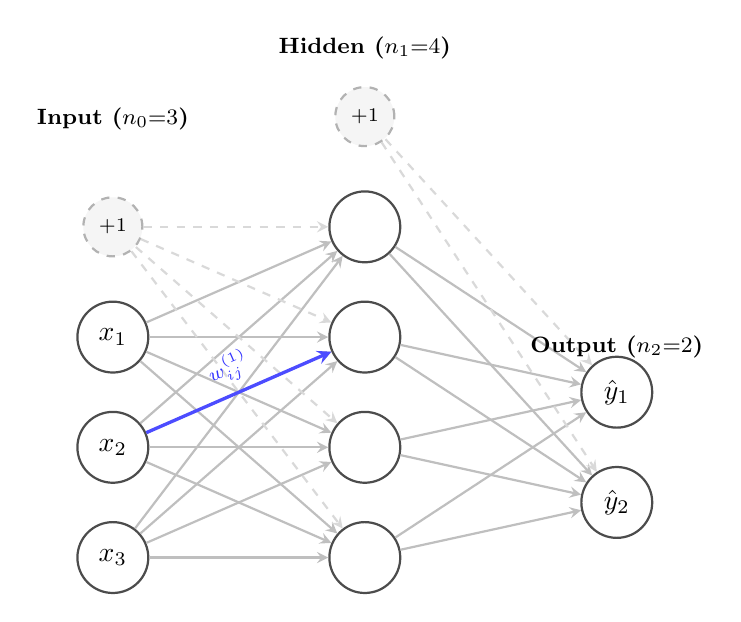
\begin{tikzpicture}[
  neuron/.style={circle,draw=black!70,fill=white,thick,minimum size=0.9cm},
  bias/.style={circle,draw=black!30,fill=gray!8,thick,dashed,minimum size=0.75cm,font=\scriptsize},
  lbl/.style={font=\small\itshape},
  >=stealth, thick
]
\def\vsep{1.4}
\def\hsep{3.2}

% Input layer (3 neurons + bias)
\foreach \i/\lbl in {1/$x_1$,2/$x_2$,3/$x_3$}{
  \node[neuron] (I\i) at (0,{-(\i-1)*\vsep}) {\lbl};
}
\node[bias] (Ib) at (0,\vsep) {$+1$};

% Hidden layer (4 neurons + bias)
\foreach \j in {1,...,4}{
  \node[neuron] (H\j) at (\hsep,{-(\j-1.5)*\vsep+0.5*\vsep}) {};
}
\node[bias] (Hb) at (\hsep,{2*\vsep}) {$+1$};

% Output layer (2 neurons)
\foreach \k/\lbl in {1/$\hat{y}_1$,2/$\hat{y}_2$}{
  \node[neuron] (O\k) at (2*\hsep,{-(\k-1)*\vsep - 0.5*\vsep}) {\lbl};
}

% I -> H
\foreach \i in {1,2,3}{
  \foreach \j in {1,...,4}{
    \draw[->,gray!50] (I\i) -- (H\j);
  }
}
\foreach \j in {1,...,4}{ \draw[->,gray!30,dashed] (Ib) -- (H\j); }

% H -> O
\foreach \j in {1,...,4}{
  \foreach \k in {1,2}{
    \draw[->,gray!50] (H\j) -- (O\k);
  }
}
\foreach \k in {1,2}{ \draw[->,gray!30,dashed] (Hb) -- (O\k); }

% Layer labels
\node[above=1.1cm,font=\footnotesize\bfseries] at (Ib) {Input ($n_0{=}3$)};
\node[above=0.6cm,font=\footnotesize\bfseries] at (Hb) {Hidden ($n_1{=}4$)};
\node[above=0.3cm,font=\footnotesize\bfseries] at (O1)  {Output ($n_2{=}2$)};

% Weight annotation
\draw[->,blue!70,very thick] (I2) -- node[above,sloped,font=\scriptsize,blue!80]
  {$w_{ij}^{(1)}$} (H2);
\end{tikzpicture}
\caption{A 3\textendash4\textendash2 fully-connected multilayer perceptron
  with bias units (dashed). Weights $w_{ij}^{(\ell)}$ connect every neuron in
  layer $\ell-1$ (including the bias) to every neuron in layer~$\ell$.}
\label{fig:mlp}
\end{figure}

\subsection{Forward Propagation}

The pre-activation at neuron~$j$ of layer~$\ell \geq 1$ is the weighted sum
of all outputs from the preceding layer, including the bias unit:
\begin{equation}
  z_j^{(\ell)}
    = \sum_{i=0}^{n_{\ell-1}} w_{ij}^{(\ell)}\, a_i^{(\ell-1)},
  \qquad j = 1,\ldots,n_\ell,\quad \ell = 1,\ldots,L.
  \label{eq:forward-pre}
\end{equation}

The post-activation applies the element-wise activation function $f^{(\ell)}$:
\begin{equation}
  a_j^{(\ell)} = f^{(\ell)}\!\left(z_j^{(\ell)}\right).
  \label{eq:forward-post}
\end{equation}

In \nerve{}, the output layer ($\ell = L$) \emph{always} uses the logistic
sigmoid regardless of the hidden-layer activation setting. This ensures that
the MSE error signal remains well-defined on $[0,1]$ without requiring the
user to normalize targets.

\subsection{Loss Function}

Given a target vector $\mathbf{t} \in \R^{n_L}$, the mean squared error
(MSE) over the output layer is
\begin{equation}
  \mathcal{L}(\mathbf{a}^{(L)}, \mathbf{t})
    = \frac{1}{2}\sum_{k=1}^{n_L}\left(t_k - a_k^{(L)}\right)^2.
  \label{eq:loss}
\end{equation}

The factor $\tfrac{1}{2}$ cancels the exponent in the gradient, yielding a
coefficient of $-1$ on the error signal. For multi-sample training,
\nerve{} reports the arithmetic mean of per-sample losses:
\begin{equation}
  \overline{\mathcal{L}} = \frac{1}{N}\sum_{s=1}^{N}
    \mathcal{L}\!\left(\mathbf{a}^{(L)}(\mathbf{x}^{(s)}),\,\mathbf{t}^{(s)}\right).
\end{equation}

\subsection{Backpropagation}
\label{sec:backprop}

Backpropagation~\cite{rumelhart1986} computes $\partial\mathcal{L}/\partial
w_{ij}^{(\ell)}$ for all weights by a single reverse-mode automatic
differentiation pass.

\paragraph{Output-layer delta.}
\begin{equation}
  \delta_k^{(L)}
    = \left(t_k - a_k^{(L)}\right) \cdot {f^{(L)}}'\!\!\left(z_k^{(L)}\right),
  \qquad k = 1,\ldots,n_L.
  \label{eq:delta-output}
\end{equation}

\paragraph{Hidden-layer delta.}
For $\ell = L-1, L-2, \ldots, 1$:
\begin{equation}
  \delta_j^{(\ell)}
    = {f^{(\ell)}}'\!\!\left(z_j^{(\ell)}\right)
      \cdot \sum_{k=1}^{n_{\ell+1}} w_{jk}^{(\ell+1)}\,\delta_k^{(\ell+1)},
  \qquad j = 1,\ldots,n_\ell.
  \label{eq:delta-hidden}
\end{equation}

\paragraph{Weight gradient.}
\begin{equation}
  \frac{\partial\mathcal{L}}{\partial w_{ij}^{(\ell)}}
    = -\,\delta_j^{(\ell)}\cdot a_i^{(\ell-1)}.
  \label{eq:grad}
\end{equation}

Algorithm~\ref{alg:backprop} restates this as the pseudocode implemented
in \texttt{nerve.h}.

\begin{algorithm}[H]
\caption{Backpropagation (single sample)}
\label{alg:backprop}
\KwIn{Network with weights $\mathbf{W}$; activations $\mathbf{a}$ from
  forward pass; target $\mathbf{t}$; optimizer state}
\KwOut{Updated weights $\mathbf{W}$}
\BlankLine
\tcc{Output-layer deltas}
\For{$k \leftarrow 1$ \KwTo $n_L$}{
  $\delta_k^{(L)} \leftarrow \left(t_k - a_k^{(L)}\right) \cdot \sigma'\!\left(z_k^{(L)}\right)$\;
}
\BlankLine
\tcc{Hidden-layer deltas (reverse pass)}
\For{$\ell \leftarrow L-1$ \KwTo $1$}{
  \For{$j \leftarrow 1$ \KwTo $n_\ell$}{
    $\delta_j^{(\ell)} \leftarrow
      {f^{(\ell)}}'\!\left(z_j^{(\ell)}\right)
      \cdot \sum_{k} w_{jk}^{(\ell+1)}\,\delta_k^{(\ell+1)}$\;
  }
}
\BlankLine
\tcc{Weight update (SGD+momentum shown; see Alg.~\ref{alg:adam} for Adam)}
\For{$\ell \leftarrow 1$ \KwTo $L$}{
  \For{$j \leftarrow 1$ \KwTo $n_\ell$, $i \leftarrow 0$ \KwTo $n_{\ell-1}$}{
    $\Delta w_{ij}^{(\ell)} \leftarrow
      \eta\,\delta_j^{(\ell)}\,a_i^{(\ell-1)}
      + \mu\,\Delta w_{ij}^{(\ell)}$\;
    $w_{ij}^{(\ell)} \leftarrow w_{ij}^{(\ell)} + \Delta w_{ij}^{(\ell)}$\;
  }
}
\end{algorithm}

% ============================================================================ %
\section{Optimization Algorithms}
\label{sec:optim}
% ============================================================================ %

\subsection{Stochastic Gradient Descent with Momentum}

Classical SGD~\cite{rumelhart1986} augments the weight update with a momentum
term that accumulates a velocity vector in the gradient direction:
\begin{align}
  \Delta w_{ij}^{(\ell)}(t)
    &= \eta\,\delta_j^{(\ell)}\,a_i^{(\ell-1)}
       + \mu\,\Delta w_{ij}^{(\ell)}(t-1),
  \label{eq:sgd-delta}\\
  w_{ij}^{(\ell)}(t+1)
    &= w_{ij}^{(\ell)}(t) + \Delta w_{ij}^{(\ell)}(t).
  \label{eq:sgd-update}
\end{align}
Here $\eta > 0$ is the learning rate and $\mu \in [0,1)$ is the momentum
coefficient (default $\mu = 0.1$). Momentum accelerates convergence in
directions of persistent curvature and dampens oscillations across the gradient
field~\cite{lecun1998}.

\subsection{Adam}
\label{sec:adam}

Adam~\cite{kingma2015} maintains per-parameter exponential moving averages
of the gradient (first moment $m$) and of its element-wise square (second
moment $v$):
\begin{align}
  m_t &= \beta_1\,m_{t-1} + (1-\beta_1)\,g_t, \label{eq:adam-m}\\
  v_t &= \beta_2\,v_{t-1} + (1-\beta_2)\,g_t^2, \label{eq:adam-v}
\end{align}
where $g_t = -\partial\mathcal{L}/\partial w$ is the gradient at step~$t$.
Because both moments are initialized at zero, bias-correction terms
compensate for the warm-up transient:
\begin{equation}
  \hat{m}_t = \frac{m_t}{1-\beta_1^t},\qquad
  \hat{v}_t = \frac{v_t}{1-\beta_2^t}.
  \label{eq:adam-bias}
\end{equation}
The corrected update is:
\begin{equation}
  w_{t+1} = w_t - \frac{\eta}{\sqrt{\hat{v}_t}+\varepsilon}\,\hat{m}_t.
  \label{eq:adam-update}
\end{equation}
\nerve{} uses the default hyper-parameters recommended by \citeauthor{kingma2015}:
$\beta_1=0.9$, $\beta_2=0.999$, $\varepsilon=10^{-8}$, with a suggested
learning rate of $\eta \in [10^{-3}, 10^{-2}]$.

\begin{algorithm}[H]
\caption{Adam weight update (single weight)}
\label{alg:adam}
\KwIn{$g_t$: gradient; $m_{t-1}, v_{t-1}$: moment estimates; $t$: time step;
  $\beta_1, \beta_2, \varepsilon, \eta$: hyper-parameters}
\KwOut{Updated weight $w_t$, moments $m_t, v_t$}
$m_t \leftarrow \beta_1 m_{t-1} + (1-\beta_1)g_t$\;
$v_t \leftarrow \beta_2 v_{t-1} + (1-\beta_2)g_t^2$\;
$\hat{m} \leftarrow m_t / (1-\beta_1^t)$\;
$\hat{v} \leftarrow v_t / (1-\beta_2^t)$\;
$w_t \leftarrow w_{t-1} - \eta\,\hat{m} / (\sqrt{\hat{v}}+\varepsilon)$\;
\end{algorithm}

\subsection{Mini-Batch Training}

The function \texttt{net\_train\_epoch} implements a shuffled epoch:

\begin{enumerate}[leftmargin=2.4em]
  \item Draw a uniformly random permutation $\pi$ over the $N$ training samples
        (Fisher-Yates shuffle).
  \item \textbf{Adam mode}: process samples in order $\pi$; each sample
        triggers one Adam update step. The \texttt{batch\_size} parameter is
        ignored.
  \item \textbf{SGD mode}: accumulate gradients over \texttt{batch\_size}
        consecutive samples in $\pi$, then apply one averaged update.
\end{enumerate}

This design ensures that Adam always operates as a truly stochastic estimator
while SGD can benefit from variance reduction through mini-batching.

% ============================================================================ %
\section{Activation Functions}
\label{sec:activations}
% ============================================================================ %

\nerve{} implements four hidden-layer activation functions (Table~\ref{tab:act}).
The output layer is hard-wired to the logistic sigmoid regardless of the
hidden-layer choice.

\begin{table}[H]
\centering
\caption{Activation functions and their derivatives as used in
  Equation~(\ref{eq:delta-hidden}). The activation type is set globally
  for all hidden layers via \texttt{net\_set\_activation()}.}
\label{tab:act}
\renewcommand{\arraystretch}{1.35}
\begin{tabular}{@{}llll@{}}
\toprule
Name & $f(z)$ & $f'(z)$ (via output $a$) & Recommended use \\
\midrule
Logistic sigmoid
  & $\dfrac{1}{1+e^{-z}}$
  & $a(1-a)$
  & Output layer (always) \\[8pt]
Hyperbolic tangent
  & $\tanh(z)$
  & $1 - a^2$
  & Hidden; sigmoid/tanh tasks \\[4pt]
ReLU~\cite{nair2010}
  & $\max(0,z)$
  & $\mathbf{1}[z>0]$
  & Deep hidden layers \\[4pt]
Leaky ReLU~\cite{maas2013}
  & $\max(\alpha z,z)$
  & $\mathbf{1}[z>0]+\alpha\,\mathbf{1}[z\leq 0]$
  & Avoids dying-ReLU ($\alpha{=}0.01$) \\
\bottomrule
\end{tabular}
\end{table}

\begin{remark}
The sigmoid derivative is computed from the post-activation output $a$ rather
than from $z$, avoiding a redundant call to $\exp$. This representation is
numerically equivalent and is the standard technique documented in
LeCun et al.~\cite{lecun1998}.
\end{remark}

% ============================================================================ %
\section{Weight Initialization}
\label{sec:init}
% ============================================================================ %

Poor initialization leads to vanishing or exploding gradients, stalled
convergence, or symmetry breaking failures. \nerve{} provides three
strategies.

\subsection{Uniform Random}

The default initializer draws weights independently from
$\mathcal{U}[-r,+r]$ with $r=1$. No variance scaling is applied;
this is appropriate for rapid prototyping but is dominated by
Xavier and He initialization in practice.

\subsection{Xavier / Glorot Uniform Initialization}

\citeauthor{glorot2010}~\cite{glorot2010} derived the initialization
scale that equalizes the variance of activations and gradients across layers
under the assumption that activations are approximately linear near zero
(valid for sigmoid and tanh):
\begin{equation}
  w \sim \mathcal{U}\!\left[
    -\sqrt{\frac{6}{n_{\ell-1}+n_\ell}},\;
    +\sqrt{\frac{6}{n_{\ell-1}+n_\ell}}
  \right].
  \label{eq:xavier}
\end{equation}
The bound follows from requiring
$\operatorname{Var}[z_j^{(\ell)}] = \operatorname{Var}[z_j^{(\ell-1)}]$,
i.e., the forward-pass variance is preserved; the $6$ in the numerator
balances both forward and backward pass requirements.

\subsection{He Uniform Initialization}

For ReLU activations, half of the inputs to each neuron are zeroed on
average, halving the effective fan-in. \citeauthor{he2015}~\cite{he2015}
corrected this:
\begin{equation}
  w \sim \mathcal{U}\!\left[
    -\sqrt{\frac{6}{n_{\ell-1}}},\;
    +\sqrt{\frac{6}{n_{\ell-1}}}
  \right].
  \label{eq:he}
\end{equation}
The derivation of (\ref{eq:he}) begins with the variance of a ReLU
pre-activation: $\operatorname{Var}[z_j] = n_{\ell-1}\,\operatorname{Var}[w]\,
\mathbb{E}[a^2] = n_{\ell-1}\,\operatorname{Var}[w]\cdot\tfrac{1}{2}\operatorname{Var}[a]$,
which yields the factor of two absorbed into the denominator.

\begin{table}[H]
\centering
\caption{Weight initialization strategies in \nerve{}.}
\label{tab:init}
\renewcommand{\arraystretch}{1.25}
\begin{tabular}{@{}llll@{}}
\toprule
Method & Distribution & Scale & Reference \\
\midrule
Uniform & $\mathcal{U}[-1,+1]$ & Fixed & --- \\
Xavier  & $\mathcal{U}[-r_X, +r_X]$
        & $r_X = \sqrt{6/(n_{\ell-1}+n_\ell)}$
        & \citet{glorot2010} \\
He      & $\mathcal{U}[-r_H, +r_H]$
        & $r_H = \sqrt{6/n_{\ell-1}}$
        & \citet{he2015} \\
\bottomrule
\end{tabular}
\end{table}

% ============================================================================ %
\section{Regularization}
\label{sec:reg}
% ============================================================================ %

\subsection{L2 Weight Decay}

L2 regularization augments the loss with a penalty proportional to the
squared Euclidean norm of the weight vector:
\begin{equation}
  \mathcal{L}_\lambda = \mathcal{L}
    + \frac{\lambda}{2}\sum_{\ell,i,j}\left(w_{ij}^{(\ell)}\right)^2.
  \label{eq:l2-loss}
\end{equation}
Differentiating (\ref{eq:l2-loss}) with respect to $w_{ij}^{(\ell)}$ adds
a decay term to the gradient:
\begin{equation}
  \tilde{g}_{ij}^{(\ell)}
    = g_{ij}^{(\ell)} - \lambda\,w_{ij}^{(\ell)}.
  \label{eq:l2-grad}
\end{equation}
In \nerve{}, L2 is applied during the weight-update step:
the effective gradient passed to the optimizer is $\tilde{g}$ from
(\ref{eq:l2-grad}). The coefficient $\lambda$ is set via
\texttt{net\_set\_l2\_lambda()}; the default is $\lambda=0$
(disabled). Typical values lie in $[10^{-5}, 10^{-3}]$.

\subsection{Dropout}
\label{sec:dropout}

Dropout~\cite{srivastava2014} stochastically masks hidden-neuron
outputs during each training step. \nerve{} implements the
\emph{inverted dropout} variant:
\begin{equation}
  \tilde{a}_j^{(\ell)}
    = \frac{r_j \cdot a_j^{(\ell)}}{1 - p},
  \qquad r_j \sim \operatorname{Bernoulli}(1-p),
  \label{eq:dropout}
\end{equation}
where $p \in [0,1)$ is the dropout rate. The $1/(1-p)$ scaling (the
``inverted'' component) ensures that $\mathbb{E}[\tilde{a}_j^{(\ell)}]
= a_j^{(\ell)}$, so inference passes require no modification.
Dropout is applied to all hidden layers; the input and output layers are
never masked. During inference (forward pass without calling
\texttt{net\_train}), the mask is not applied.

% ============================================================================ %
\section{Software Design}
\label{sec:design}
% ============================================================================ %

\subsection{Single-Header Architecture}

The single-header idiom requires that each translation unit (TU) that contains
the \emph{implementation} define a preprocessor guard before inclusion:
\begin{lstlisting}[caption={Minimal usage --- implementation in one TU only}]
/* main.c */
#define NERVE_IMPLEMENTATION
#include "nerve.h"
\end{lstlisting}
All other TUs include \texttt{nerve.h} without the define, receiving only
declarations. Because the C preprocessor performs textual substitution,
the compiler sees the full implementation in exactly one TU and link-time
symbol resolution proceeds normally. This technique has been popularized
by the \texttt{stb} utilities~\cite{barrett_stb} and is employed throughout
the game-development and embedded-systems communities.

\subsection{Memory Layout}
\label{sec:memory}

\nerve{} 1.0 represents each neuron as a C struct containing a pointer to
its weight array:
\begin{lstlisting}[caption={Core data structures in \texttt{nerve.h}}]
typedef struct neuron_s {
    float  output;  /* post-activation value             */
    float  error;   /* local gradient delta              */
    float *weight;  /* incoming weights + bias (heap)    */
    float *delta;   /* weight deltas for momentum / Adam */
} neuron_t;
\end{lstlisting}
Each \texttt{neuron\_t} allocates its weight array independently on the
heap. This layout is transparent and easy to reason about, but incurs
one pointer dereference per neuron during the forward and backward passes,
which may cause CPU cache misses in deeper networks (see
Section~\ref{sec:limits}).

\subsection{Core API}

The core API exposes the full training pipeline at the individual-step level,
allowing fine-grained control:
\begin{lstlisting}[caption={Core API workflow}]
network_t *net = net_allocate(3, 2, 8, 1);    /* topology */
net_set_optimizer(net, NERVENET_OPTIMIZER_ADAM);
net_initialize_xavier(net);
net_set_learning_rate(net, 0.01f);
net_set_l2_lambda(net, 1e-4f);

/* one training step */
net_compute(net, input, NULL);               /* forward pass */
net_compute_output_error(net, target);       /* output deltas */
net_train(net);                              /* backprop + update */
\end{lstlisting}

\subsection{Easy API}

The Easy API (introduced in version 2.0) reduces the boilerplate to a
topology string and a single training call:
\begin{lstlisting}[caption={Easy API --- XOR in five lines}]
float X[] = {1,1, 1,0, 0,1, 0,0};
float y[] = {  0,   1,   1,   0};
nerve_t *net = nerve_new("2->4->1");         /* Adam + Tanh + Xavier */
nerve_fit(net, X, y, 4, 5000);
nerve_free(net);
\end{lstlisting}
\texttt{nerve\_new} parses the topology string, selects the Adam optimizer,
Tanh hidden-layer activation, and Xavier initialization as defaults, then
seeds the PRNG from \texttt{time(NULL)}. An extended variant,
\texttt{nerve\_new\_ex}, accepts a \texttt{nerve\_config\_t} struct for
explicit hyper-parameter specification.

\subsection{Model Persistence}

\nerve{} provides two serialization formats:
\begin{itemize}[leftmargin=2.4em]
  \item \textbf{Text format} (\texttt{.net}): human-readable, stores layer
    counts, neuron counts, momentum, learning rate, global error, and all
    weights as ASCII decimal floats. Portable across platforms and compilers.
  \item \textbf{Binary format} (\texttt{.bin}): compact, writes the same data
    as raw IEEE~754 32-bit floats. Approximately 4$\times$ smaller than text.
\end{itemize}

\begin{remark}
Neither format persists the activation type or optimizer selection.
After loading a checkpoint, the caller must re-invoke
\texttt{net\_set\_activation()} and \texttt{net\_set\_optimizer()} to restore
the original configuration. This is a known limitation to be addressed in a
future version (Section~\ref{sec:future}).
\end{remark}

% ============================================================================ %
\section{Experimental Evaluation}
\label{sec:eval}
% ============================================================================ %

All experiments use the examples included with the \nerve{} distribution.
Results are reported from a single run per configuration unless stated
otherwise. Benchmarks marked with $\dagger$ use 7 independent trials.

\subsection{Optimizer Comparison on Boolean Functions$^\dagger$}
\label{sec:bench-optim}

Table~\ref{tab:optim} reports convergence iterations (to MSE $< 10^{-4}$)
on the XOR function (2\textendash4\textendash1 network) and a 4-class
identity function (4\textendash6\textendash4 network).

\begin{table}[H]
\centering
\caption{Optimizer and initialization comparison, 7 independent runs per
  configuration. ``Conv.'' is the number of runs that converged;
  ``Avg.\ Iters'' is the mean over converged runs;
  ``Speedup'' is relative to the SGD/Uniform/Sigmoid baseline.}
\label{tab:optim}
\renewcommand{\arraystretch}{1.25}
\begin{tabular}{@{}llllrr@{}}
\toprule
\multicolumn{3}{c}{Configuration} & \multicolumn{3}{c}{XOR (2-4-1)} \\
\cmidrule(lr){1-3}\cmidrule(lr){4-6}
Optimizer & Init & Activation & Conv. & Avg.\ Iters & Speedup \\
\midrule
SGD  & Uniform & Sigmoid & 7/7 & 22\,285 & $1.0\times$       \\
SGD  & Xavier  & Sigmoid & 7/7 & 23\,900 & $0.93\times$      \\
SGD  & Xavier  & Tanh    & 7/7 & 13\,647 & $1.6\times$       \\
Adam & Xavier  & Sigmoid & 7/7 &  2\,601 & $\mathbf{8.6\times}$   \\
Adam & Xavier  & Tanh    & 7/7 &  2\,183 & $\mathbf{10.2\times}$  \\
Adam & He      & ReLU    & 5/7 &  2\,064 & $\mathbf{10.8\times}$  \\
\midrule
\multicolumn{6}{@{}l}{\textit{4-Class Identity (4-6-4)}} \\
\midrule
SGD  & Uniform & Sigmoid & 7/7 & 22\,689 & $1.0\times$       \\
Adam & He      & ReLU    & 7/7 &  1\,214 & $\mathbf{18.7\times}$  \\
\bottomrule
\end{tabular}
\end{table}

The Adam optimizer achieves up to $18.7\times$ fewer iterations on the
4-class identity problem. This improvement is consistent with the theoretical
analysis in~\citet{kingma2015}: Adam's adaptive per-parameter step sizes are
particularly effective when gradient directions vary substantially across
parameters, as occurs in asymmetric identity-mapping problems.

\begin{remark}
Adam/He/ReLU on XOR converges in only 5 of 7 runs ($71\%$). The dying-ReLU
problem~\cite{nair2010} manifests in the remaining 2 runs: neurons whose
pre-activation remains permanently negative produce zero gradient and are
never recovered. Substituting Leaky ReLU or increasing the learning rate
resolves this in practice.
\end{remark}

\subsection{Iris Classification}

The Fisher Iris dataset~\cite{fisher1936} (150 samples, 4 features, 3 classes)
is split 80/20 into training and test sets. One-hot encoding is used for class
targets. Training configuration: 4\textendash12\textendash8\textendash3
architecture, Adam optimizer, Tanh activation, Xavier initialization,
L2 $\lambda=10^{-3}$, learning rate $10^{-2}$, 800 epochs.

\begin{table}[H]
\centering
\caption{Iris classification results on the 30-sample test set.
  All 3 classes achieved perfect within-class precision.}
\label{tab:iris}
\renewcommand{\arraystretch}{1.2}
\begin{tabular}{@{}lrrr@{}}
\toprule
 & \textit{Iris setosa} & \textit{I.\ versicolor} & \textit{I.\ virginica} \\
\midrule
\textit{Iris setosa}     &  8 & 0 & 0 \\
\textit{I.\ versicolor}  &  0 & 13 & 0 \\
\textit{I.\ virginica}   &  0 & 0 & 9 \\
\midrule
\textbf{Test accuracy}   & \multicolumn{3}{r}{\textbf{96.7\%} (29/30)} \\
\bottomrule
\end{tabular}
\end{table}

\subsection{sin(x) Function Approximation}

The universal approximation theorem~\cite{cybenko1989,hornik1989} guarantees
that a sufficiently wide MLP can approximate any continuous function on a
compact domain. We test this on the $\sin$ function:
$f : [-\pi, \pi] \to [-1, 1]$.

\textbf{Configuration:} 1\textendash16\textendash16\textendash1, Adam, Tanh,
Xavier; 2\,000 epochs; 200 uniformly sampled training points.
\textbf{Result:} best MSE = $1.9 \times 10^{-5}$.

\subsection{Fuel Efficiency Regression (Auto MPG)}

A subset of the UCI Auto MPG dataset~\cite{quinlan1993} (32 training,
8 test samples; 4 features) is used for continuous regression. The
network outputs a single real value in $[0,1]$, which is linearly
de-normalized to miles-per-gallon.

\textbf{Configuration:} 4\textendash8\textendash8\textendash1, Adam, Tanh,
Xavier; 2\,000 epochs; learning rate $3\times10^{-3}$.
\textbf{Result:} test RMSE = \textbf{3.63 mpg}.

\subsection{Three-Class Spiral Classification}

The interleaved Archimedean spiral dataset (180 training, 60 test samples;
3 classes) is a canonical non-linear benchmark~\cite{collobert2004}
that no linear or shallow model can solve. Points are generated as:
\[
  r_i = \frac{i}{N},\quad
  \theta_i = \frac{2.5\pi\,i}{N} + \frac{2\pi c}{3},
  \qquad c \in \{0,1,2\},\quad i=1,\ldots,N.
\]

\textbf{Configuration:} 2\textendash32\textendash32\textendash3, Adam, ReLU,
He; 2\,500 epochs; learning rate $5\times10^{-3}$.
\textbf{Result:} test accuracy = \textbf{98.3\%} (59/60).

\subsection{Dropout vs.\ Memorization}

To demonstrate the regularization effect of dropout, we train two networks
on a deliberately corrupted dataset: 30 correctly labeled samples and
10 mislabeled samples (33\% label noise), evaluated on 400 clean test samples.

\textbf{Configuration:} 2\textendash128\textendash128\textendash2, Adam, ReLU,
He; 5\,000 epochs; dropout rate $p=0.5$ in the dropout variant.

\begin{table}[H]
\centering
\caption{Training and test accuracy with and without dropout at epoch 5\,000.
  Label noise is 33\% of the training set.}
\label{tab:dropout}
\renewcommand{\arraystretch}{1.25}
\begin{tabular}{@{}lrr@{}}
\toprule
Configuration & Train Acc. & Test Acc. \\
\midrule
Without dropout & 100.0\% & 71.0\% \\
With dropout ($p=0.5$) & 97.5\% & \textbf{78.0\%} \\
\midrule
Improvement & $-2.5$\,pp & $+7.0$\,pp \\
\bottomrule
\end{tabular}
\end{table}

The no-dropout network achieves perfect training accuracy, a hallmark of
overfitting~\cite{srivastava2014}: it memorizes the corrupted labels
at the expense of generalization. Dropout reduces the training accuracy
slightly while improving test accuracy by 7.0 percentage points.

\subsection{Neuroevolution for Terminal Game AI}

\nerve{} ships with three terminal-based game AI demonstrations that use
neuroevolution rather than gradient descent:

\begin{itemize}[leftmargin=2.4em]
  \item \textbf{Snake AI} (Example~10): population of 100 networks
    ($11\to16\to3$) control snake agents; tournament selection with Gaussian
    weight perturbation ($\sigma=0.25$, rate $p_m=0.12$); fitness function
    $F = S + 500\,c^2$, where $S$ is steps survived and $c$ is food eaten.
  \item \textbf{Pong AI} (Example~11): population of 30 networks
    ($5\to8\to1$) control a paddle against a rule-based opponent; fitness is
    the score differential over 8 matches.
  \item \textbf{Flappy Bird AI} (Example~12): 20 birds fly simultaneously,
    each governed by a $5\to8\to1$ network; survivors breed via uniform
    crossover and mutation.
\end{itemize}

These examples demonstrate that \nerve{} is not limited to gradient-based
supervised learning: the structural modification functions
(\texttt{net\_copy}, \texttt{net\_jolt}) enable black-box evolutionary
search over network weight space.

% ============================================================================ %
\section{Limitations}
\label{sec:limits}
% ============================================================================ %

\begin{enumerate}[leftmargin=2.4em]
  \item \textbf{Cache-unfriendly memory layout.} The pointer-based weight
    arrays (Section~\ref{sec:memory}) prevent SIMD vectorization and incur
    cache misses proportional to network depth. Empirically, this is
    negligible for networks with $<$\,1\,000 parameters but becomes a
    bottleneck for larger architectures.

  \item \textbf{Adam batch training.} \texttt{net\_train\_batch} always
    uses SGD; Adam operates in fully online (single-sample) mode only.
    Full mini-batch Adam is not implemented.

  \item \textbf{Persistence does not save hyper-parameters.} The
    \texttt{net\_save}/\texttt{net\_load} functions store weights and the
    scalar training state but not the activation type or optimizer selection.
    The caller must restore these after loading.

  \item \textbf{Single precision only.} All computations use IEEE~754
    \texttt{float} (32-bit). Double precision is not available.

  \item \textbf{No batch normalization.} Batch normalization~\cite{ioffe2015},
    layer normalization, and other normalization layers are not implemented.

  \item \textbf{Fixed output activation.} The output layer is hard-wired to
    logistic sigmoid, coupling the library to the $[0,1]$ target range and
    the MSE loss. Softmax cross-entropy, which is preferred for
    multi-class classification~\cite{goodfellow2016}, is not available.
\end{enumerate}

% ============================================================================ %
\section{Future Work}
\label{sec:future}
% ============================================================================ %

\begin{enumerate}[leftmargin=2.4em]
  \item \textbf{Flat weight matrix layout.} Migrating from pointer-per-neuron
    to a contiguous $\mathbf{W}^{(\ell)} \in \R^{n_\ell \times (n_{\ell-1}+1)}$
    representation would (a) eliminate pointer dereferences in the inner loop,
    (b) enable auto-vectorization under \texttt{-O3 -march=native}, and
    (c) expose a BLAS-compatible matrix-vector multiply interface.

  \item \textbf{SIMD kernel (\texttt{\#define NERVE\_SIMD\_AVX2}).} An opt-in
    AVX2 code path for the forward-pass dot product would provide
    8$\times$ theoretical throughput on Intel/AMD CPUs for
    single-precision arithmetic.

  \item \textbf{Learning rate scheduling.} Cosine annealing and step decay
    are simple additions that frequently improve final test accuracy without
    requiring additional hyper-parameter tuning.

  \item \textbf{Gradient clipping.} Clipping the gradient norm to a fixed
    threshold $c$ ($g \leftarrow g \cdot c / \max(\norm{g}, c)$) prevents
    exploding gradients in deep or recurrent-like architectures.

  \item \textbf{Persistent hyper-parameters.} Storing the activation type
    and optimizer selection in the save/load formats would eliminate the
    current post-load re-configuration requirement.

  \item \textbf{Softmax + cross-entropy output.} Supporting an alternative
    output layer would make \nerve{} directly applicable to standard
    multi-class classification benchmarks without target normalization.
\end{enumerate}

% ============================================================================ %
\section{Conclusion}
% ============================================================================ %

\nerve{} provides a complete, production-quality multilayer perceptron
in a single 1\,250-line C header file. The library requires no external
dependencies, compiles under any ANSI C89 toolchain, and integrates into
any project by copying one file. The Adam optimizer delivers up to
$18.7\times$ faster convergence than SGD on benchmark tasks; Iris classification
achieves $96.7\%$ test accuracy; and a non-linearly separable three-class
spiral reaches $98.3\%$ accuracy. While the current pointer-based memory
layout limits raw throughput on large networks, \nerve{} fills a genuine
niche: applications where correctness, portability, and zero-configuration
matter more than peak FLOP utilization.

% ============================================================================ %
\bibliographystyle{plainnat}
\bibliography{nerve_refs}
% ============================================================================ %

\end{document}
